%% bare_adv.tex
%% V1.4b
%% 2015/08/26
%% by Michael Shell
%% See:
%% http://www.michaelshell.org/
%% for current contact information.
%%
%% This is a skeleton file demonstrating the advanced use of IEEEtran.cls
%% (requires IEEEtran.cls version 1.8b or later) with an IEEE Computer
%% Society journal paper.
%%
%% Support sites:
%% http://www.michaelshell.org/tex/ieeetran/
%% http://www.ctan.org/pkg/ieeetran
%% and
%% http://www.ieee.org/

%%*************************************************************************
%% Legal Notice:
%% This code is offered as-is without any warranty either expressed or
%% implied; without even the implied warranty of MERCHANTABILITY or
%% FITNESS FOR A PARTICULAR PURPOSE!
%% User assumes all risk.
%% In no event shall the IEEE or any contributor to this code be liable for
%% any damages or losses, including, but not limited to, incidental,
%% consequential, or any other damages, resulting from the use or misuse
%% of any information contained here.
%%
%% All comments are the opinions of their respective authors and are not
%% necessarily endorsed by the IEEE.
%%
%% This work is distributed under the LaTeX Project Public License (LPPL)
%% ( http://www.latex-project.org/ ) version 1.3, and may be freely used,
%% distributed and modified. A copy of the LPPL, version 1.3, is included
%% in the base LaTeX documentation of all distributions of LaTeX released
%% 2003/12/01 or later.
%% Retain all contribution notices and credits.
%% ** Modified files should be clearly indicated as such, including  **
%% ** renaming them and changing author support contact information. **
%%*************************************************************************


% *** Authors should verify (and, if needed, correct) their LaTeX system  ***
% *** with the testflow diagnostic prior to trusting their LaTeX platform ***
% *** with production work. The IEEE's font choices and paper sizes can   ***
% *** trigger bugs that do not appear when using other class files.       ***                          ***
% The testflow support page is at:
% http://www.michaelshell.org/tex/testflow/


% IEEEtran V1.7 and later provides for these CLASSINPUT macros to allow the
% user to reprogram some IEEEtran.cls defaults if needed. These settings
% override the internal defaults of IEEEtran.cls regardless of which class
% options are used. Do not use these unless you have good reason to do so as
% they can result in nonIEEE compliant documents. User beware. ;)
%
%\newcommand{\CLASSINPUTbaselinestretch}{1.0} % baselinestretch
%\newcommand{\CLASSINPUTinnersidemargin}{1in} % inner side margin
%\newcommand{\CLASSINPUToutersidemargin}{1in} % outer side margin
%\newcommand{\CLASSINPUTtoptextmargin}{1in}   % top text margin
%\newcommand{\CLASSINPUTbottomtextmargin}{1in}% bottom text margin




%
\documentclass[10pt,journal,compsoc]{IEEEtran}
% If IEEEtran.cls has not been installed into the LaTeX system files,
% manually specify the path to it like:
% \documentclass[10pt,journal,compsoc]{../sty/IEEEtran}


% For Computer Society journals, IEEEtran defaults to the use of
% Palatino/Palladio as is done in IEEE Computer Society journals.
% To go back to Times Roman, you can use this code:
%\renewcommand{\rmdefault}{ptm}\selectfont





% Some very useful LaTeX packages include:
% (uncomment the ones you want to load)



% *** MISC UTILITY PACKAGES ***
%
%\usepackage{ifpdf}
% Heiko Oberdiek's ifpdf.sty is very useful if you need conditional
% compilation based on whether the output is pdf or dvi.
% usage:
% \ifpdf
%   % pdf code
% \else
%   % dvi code
% \fi
% The latest version of ifpdf.sty can be obtained from:
% http://www.ctan.org/pkg/ifpdf
% Also, note that IEEEtran.cls V1.7 and later provides a builtin
% \ifCLASSINFOpdf conditional that works the same way.
% When switching from latex to pdflatex and vice-versa, the compiler may
% have to be run twice to clear warning/error messages.
\usepackage{pdflscape}





% *** CITATION PACKAGES ***
%
\usepackage[
backend=biber,
style=numeric,
sorting=none
]{biblatex}

\addbibresource{sources.bib}


% *** GRAPHICS RELATED PACKAGES ***

  \usepackage[pdftex]{graphicx}
  % declare the path(s) where your graphic files are
  \graphicspath{{img/}}
  % and their extensions so you won't have to specify these with
  % every instance of \includegraphics
  \DeclareGraphicsExtensions{.jpeg,.png,.jpg}





% *** MATH PACKAGES ***
%
%\usepackage{amsmath}
% A popular package from the American Mathematical Society that provides
% many useful and powerful commands for dealing with mathematics.
%
% Note that the amsmath package sets \interdisplaylinepenalty to 10000
% thus preventing page breaks from occurring within multiline equations. Use:
%\interdisplaylinepenalty=2500
% after loading amsmath to restore such page breaks as IEEEtran.cls normally
% does. amsmath.sty is already installed on most LaTeX systems. The latest
% version and documentation can be obtained at:
% http://www.ctan.org/pkg/amsmath





% *** SPECIALIZED LIST PACKAGES ***
%\usepackage{acronym}
% acronym.sty was written by Tobias Oetiker. This package provides tools for
% managing documents with large numbers of acronyms. (You don't *have* to
% use this package - unless you have a lot of acronyms, you may feel that
% such package management of them is bit of an overkill.)
% Do note that the acronym environment (which lists acronyms) will have a
% problem when used under IEEEtran.cls because acronym.sty relies on the
% description list environment - which IEEEtran.cls has customized for
% producing IEEE style lists. A workaround is to declared the longest
% label width via the IEEEtran.cls \IEEEiedlistdecl global control:
%
% \renewcommand{\IEEEiedlistdecl}{\IEEEsetlabelwidth{SONET}}
% \begin{acronym}
%
% \end{acronym}
% \renewcommand{\IEEEiedlistdecl}{\relax}% remember to reset \IEEEiedlistdecl
%
% instead of using the acronym environment's optional argument.
% The latest version and documentation can be obtained at:
% http://www.ctan.org/pkg/acronym


%\usepackage{algorithmic}
% algorithmic.sty was written by Peter Williams and Rogerio Brito.
% This package provides an algorithmic environment fo describing algorithms.
% You can use the algorithmic environment in-text or within a figure
% environment to provide for a floating algorithm. Do NOT use the algorithm
% floating environment provided by algorithm.sty (by the same authors) or
% algorithm2e.sty (by Christophe Fiorio) as the IEEE does not use dedicated
% algorithm float types and packages that provide these will not provide
% correct IEEE style captions. The latest version and documentation of
% algorithmic.sty can be obtained at:
% http://www.ctan.org/pkg/algorithms
% Also of interest may be the (relatively newer and more customizable)
% algorithmicx.sty package by Szasz Janos:
% http://www.ctan.org/pkg/algorithmicx




% *** ALIGNMENT PACKAGES ***
%
%\usepackage{array}
% Frank Mittelbach's and David Carlisle's array.sty patches and improves
% the standard LaTeX2e array and tabular environments to provide better
% appearance and additional user controls. As the default LaTeX2e table
% generation code is lacking to the point of almost being broken with
% respect to the quality of the end results, all users are strongly
% advised to use an enhanced (at the very least that provided by array.sty)
% set of table tools. array.sty is already installed on most systems. The
% latest version and documentation can be obtained at:
% http://www.ctan.org/pkg/array


%\usepackage{mdwmath}
%\usepackage{mdwtab}
% Also highly recommended is Mark Wooding's extremely powerful MDW tools,
% especially mdwmath.sty and mdwtab.sty which are used to format equations
% and tables, respectively. The MDWtools set is already installed on most
% LaTeX systems. The lastest version and documentation is available at:
% http://www.ctan.org/pkg/mdwtools


% IEEEtran contains the IEEEeqnarray family of commands that can be used to
% generate multiline equations as well as matrices, tables, etc., of high
% quality.


%\usepackage{eqparbox}
% Also of notable interest is Scott Pakin's eqparbox package for creating
% (automatically sized) equal width boxes - aka "natural width parboxes".
% Available at:
% http://www.ctan.org/pkg/eqparbox




% *** SUBFIGURE PACKAGES ***
\ifCLASSOPTIONcompsoc
  \usepackage[caption=false,font=footnotesize,labelfont=sf,textfont=sf]{subfig}
\else
  \usepackage[caption=false,font=footnotesize]{subfig}
\fi
% subfig.sty, written by Steven Douglas Cochran, is the modern replacement
% for subfigure.sty, the latter of which is no longer maintained and is
% incompatible with some LaTeX packages including fixltx2e. However,
% subfig.sty requires and automatically loads Axel Sommerfeldt's caption.sty
% which will override IEEEtran.cls' handling of captions and this will result
% in non-IEEE style figure/table captions. To prevent this problem, be sure
% and invoke subfig.sty's "caption=false" package option (available since
% subfig.sty version 1.3, 2005/06/28) as this is will preserve IEEEtran.cls
% handling of captions.
% Note that the Computer Society format requires a sans serif font rather
% than the serif font used in traditional IEEE formatting and thus the need
% to invoke different subfig.sty package options depending on whether
% compsoc mode has been enabled.
%
% The latest version and documentation of subfig.sty can be obtained at:
% http://www.ctan.org/pkg/subfig




% *** FLOAT PACKAGES ***
%
%\usepackage{fixltx2e}
% fixltx2e, the successor to the earlier fix2col.sty, was written by
% Frank Mittelbach and David Carlisle. This package corrects a few problems
% in the LaTeX2e kernel, the most notable of which is that in current
% LaTeX2e releases, the ordering of single and double column floats is not
% guaranteed to be preserved. Thus, an unpatched LaTeX2e can allow a
% single column figure to be placed prior to an earlier double column
% figure.
% Be aware that LaTeX2e kernels dated 2015 and later have fixltx2e.sty's
% corrections already built into the system in which case a warning will
% be issued if an attempt is made to load fixltx2e.sty as it is no longer
% needed.
% The latest version and documentation can be found at:
% http://www.ctan.org/pkg/fixltx2e


%\usepackage{stfloats}
% stfloats.sty was written by Sigitas Tolusis. This package gives LaTeX2e
% the ability to do double column floats at the bottom of the page as well
% as the top. (e.g., "\begin{figure*}[!b]" is not normally possible in
% LaTeX2e). It also provides a command:
%\fnbelowfloat
% to enable the placement of footnotes below bottom floats (the standard
% LaTeX2e kernel puts them above bottom floats). This is an invasive package
% which rewrites many portions of the LaTeX2e float routines. It may not work
% with other packages that modify the LaTeX2e float routines. The latest
% version and documentation can be obtained at:
% http://www.ctan.org/pkg/stfloats
% Do not use the stfloats baselinefloat ability as the IEEE does not allow
% \baselineskip to stretch. Authors submitting work to the IEEE should note
% that the IEEE rarely uses double column equations and that authors should try
% to avoid such use. Do not be tempted to use the cuted.sty or midfloat.sty
% packages (also by Sigitas Tolusis) as the IEEE does not format its papers in
% such ways.
% Do not attempt to use stfloats with fixltx2e as they are incompatible.
% Instead, use Morten Hogholm'a dblfloatfix which combines the features
% of both fixltx2e and stfloats:
%
% \usepackage{dblfloatfix}
% The latest version can be found at:
% http://www.ctan.org/pkg/dblfloatfix


%\ifCLASSOPTIONcaptionsoff
%  \usepackage[nomarkers]{endfloat}
% \let\MYoriglatexcaption\caption
% \renewcommand{\caption}[2][\relax]{\MYoriglatexcaption[#2]{#2}}
%\fi
% endfloat.sty was written by James Darrell McCauley, Jeff Goldberg and
% Axel Sommerfeldt. This package may be useful when used in conjunction with
% IEEEtran.cls'  captionsoff option. Some IEEE journals/societies require that
% submissions have lists of figures/tables at the end of the paper and that
% figures/tables without any captions are placed on a page by themselves at
% the end of the document. If needed, the draftcls IEEEtran class option or
% \CLASSINPUTbaselinestretch interface can be used to increase the line
% spacing as well. Be sure and use the nomarkers option of endfloat to
% prevent endfloat from "marking" where the figures would have been placed
% in the text. The two hack lines of code above are a slight modification of
% that suggested by in the endfloat docs (section 8.4.1) to ensure that
% the full captions always appear in the list of figures/tables - even if
% the user used the short optional argument of \caption[]{}.
% IEEE papers do not typically make use of \caption[]'s optional argument,
% so this should not be an issue. A similar trick can be used to disable
% captions of packages such as subfig.sty that lack options to turn off
% the subcaptions:
% For subfig.sty:
% \let\MYorigsubfloat\subfloat
% \renewcommand{\subfloat}[2][\relax]{\MYorigsubfloat[]{#2}}
% However, the above trick will not work if both optional arguments of
% the \subfloat command are used. Furthermore, there needs to be a
% description of each subfigure *somewhere* and endfloat does not add
% subfigure captions to its list of figures. Thus, the best approach is to
% avoid the use of subfigure captions (many IEEE journals avoid them anyway)
% and instead reference/explain all the subfigures within the main caption.
% The latest version of endfloat.sty and its documentation can obtained at:
% http://www.ctan.org/pkg/endfloat
%
% The IEEEtran \ifCLASSOPTIONcaptionsoff conditional can also be used
% later in the document, say, to conditionally put the References on a
% page by themselves.





% *** PDF, URL AND HYPERLINK PACKAGES ***
%
%\usepackage{url}
% url.sty was written by Donald Arseneau. It provides better support for
% handling and breaking URLs. url.sty is already installed on most LaTeX
% systems. The latest version and documentation can be obtained at:
% http://www.ctan.org/pkg/url
% Basically, \url{my_url_here}.


% NOTE: PDF thumbnail features are not required in IEEE papers
%       and their use requires extra complexity and work.
%\ifCLASSINFOpdf
%  \usepackage[pdftex]{thumbpdf}
%\else
%  \usepackage[dvips]{thumbpdf}
%\fi
% thumbpdf.sty and its companion Perl utility were written by Heiko Oberdiek.
% It allows the user a way to produce PDF documents that contain fancy
% thumbnail images of each of the pages (which tools like acrobat reader can
% utilize). This is possible even when using dvi->ps->pdf workflow if the
% correct thumbpdf driver options are used. thumbpdf.sty incorporates the
% file containing the PDF thumbnail information (filename.tpm is used with
% dvips, filename.tpt is used with pdftex, where filename is the base name of
% your tex document) into the final ps or pdf output document. An external
% utility, the thumbpdf *Perl script* is needed to make these .tpm or .tpt
% thumbnail files from a .ps or .pdf version of the document (which obviously
% does not yet contain pdf thumbnails). Thus, one does a:
%
% thumbpdf filename.pdf
%
% to make a filename.tpt, and:
%
% thumbpdf --mode dvips filename.ps
%
% to make a filename.tpm which will then be loaded into the document by
% thumbpdf.sty the NEXT time the document is compiled (by pdflatex or
% latex->dvips->ps2pdf). Users must be careful to regenerate the .tpt and/or
% .tpm files if the main document changes and then to recompile the
% document to incorporate the revised thumbnails to ensure that thumbnails
% match the actual pages. It is easy to forget to do this!
%
% Unix systems come with a Perl interpreter. However, MS Windows users
% will usually have to install a Perl interpreter so that the thumbpdf
% script can be run. The Ghostscript PS/PDF interpreter is also required.
% See the thumbpdf docs for details. The latest version and documentation
% can be obtained at.
% http://www.ctan.org/pkg/thumbpdf


% NOTE: PDF hyperlink and bookmark features are not required in IEEE
%       papers and their use requires extra complexity and work.
% *** IF USING HYPERREF BE SURE AND CHANGE THE EXAMPLE PDF ***
% *** TITLE/SUBJECT/AUTHOR/KEYWORDS INFO BELOW!!           ***
\newcommand\MYhyperrefoptions{bookmarks=true,bookmarksnumbered=true,
pdfpagemode={UseOutlines},plainpages=false,pdfpagelabels=true,
colorlinks=true,linkcolor={black},citecolor={black},urlcolor={black},
pdftitle={Bare Demo of IEEEtran.cls for Computer Society Journals},%<!CHANGE!
pdfsubject={Typesetting},%<!CHANGE!
pdfauthor={Michael D. Shell},%<!CHANGE!
pdfkeywords={Computer Society, IEEEtran, journal, LaTeX, paper,
             template}}%<^!CHANGE!
%\ifCLASSINFOpdf
%\usepackage[\MYhyperrefoptions,pdftex]{hyperref}
%\else
%\usepackage[\MYhyperrefoptions,breaklinks=true,dvips]{hyperref}
%\usepackage{breakurl}
%\fi
% One significant drawback of using hyperref under DVI output is that the
% LaTeX compiler cannot break URLs across lines or pages as can be done
% under pdfLaTeX's PDF output via the hyperref pdftex driver. This is
% probably the single most important capability distinction between the
% DVI and PDF output. Perhaps surprisingly, all the other PDF features
% (PDF bookmarks, thumbnails, etc.) can be preserved in
% .tex->.dvi->.ps->.pdf workflow if the respective packages/scripts are
% loaded/invoked with the correct driver options (dvips, etc.).
% As most IEEE papers use URLs sparingly (mainly in the references), this
% may not be as big an issue as with other publications.
%
% That said, Vilar Camara Neto created his breakurl.sty package which
% permits hyperref to easily break URLs even in dvi mode.
% Note that breakurl, unlike most other packages, must be loaded
% AFTER hyperref. The latest version of breakurl and its documentation can
% be obtained at:
% http://www.ctan.org/pkg/breakurl
% breakurl.sty is not for use under pdflatex pdf mode.
%
% The advanced features offer by hyperref.sty are not required for IEEE
% submission, so users should weigh these features against the added
% complexity of use.
% The package options above demonstrate how to enable PDF bookmarks
% (a type of table of contents viewable in Acrobat Reader) as well as
% PDF document information (title, subject, author and keywords) that is
% viewable in Acrobat reader's Document_Properties menu. PDF document
% information is also used extensively to automate the cataloging of PDF
% documents. The above set of options ensures that hyperlinks will not be
% colored in the text and thus will not be visible in the printed page,
% but will be active on "mouse over". USING COLORS OR OTHER HIGHLIGHTING
% OF HYPERLINKS CAN RESULT IN DOCUMENT REJECTION BY THE IEEE, especially if
% these appear on the "printed" page. IF IN DOUBT, ASK THE RELEVANT
% SUBMISSION EDITOR. You may need to add the option hypertexnames=false if
% you used duplicate equation numbers, etc., but this should not be needed
% in normal IEEE work.
% The latest version of hyperref and its documentation can be obtained at:
% http://www.ctan.org/pkg/hyperref





% *** Do not adjust lengths that control margins, column widths, etc. ***
% *** Do not use packages that alter fonts (such as pslatex).         ***
% There should be no need to do such things with IEEEtran.cls V1.6 and later.
% (Unless specifically asked to do so by the journal or conference you plan
% to submit to, of course. )


% correct bad hyphenation here
\hyphenation{op-tical net-works semi-conduc-tor}


\begin{document}
%
% paper title
% Titles are generally capitalized except for words such as a, an, and, as,
% at, but, by, for, in, nor, of, on, or, the, to and up, which are usually
% not capitalized unless they are the first or last word of the title.
% Linebreaks \\ can be used within to get better formatting as desired.
% Do not put math or special symbols in the title.
\title{Earbeamer: A Parallel Beamforming Hearing Aid System}
%
%
% author names and IEEE memberships
% note positions of commas and nonbreaking spaces ( ~ ) LaTeX will not break
% a structure at a ~ so this keeps an author's name from being broken across
% two lines.
% use \thanks{} to gain access to the first footnote area
% a separate \thanks must be used for each paragraph as LaTeX2e's \thanks
% was not built to handle multiple paragraphs
%
%
%\IEEEcompsocitemizethanks is a special \thanks that produces the bulleted
% lists the Computer Society journals use for "first footnote" author
% affiliations. Use \IEEEcompsocthanksitem which works much like \item
% for each affiliation group. When not in compsoc mode,
% \IEEEcompsocitemizethanks becomes like \thanks and
% \IEEEcompsocthanksitem becomes a line break with idention. This
% facilitates dual compilation, although admittedly the differences in the
% desired content of \author between the different types of papers makes a
% one-size-fits-all approach a daunting prospect. For instance, compsoc
% journal papers have the author affiliations above the "Manuscript
% received ..."  text while in non-compsoc journals this is reversed. Sigh.

\author{Niket~Gupta,~CSE,
        Aaron~Lucia,~CSE,
        Nathan~Dunn,~CSE,
        and~Matteo~Puzella,~EE% <-this % stops a space
}

% note the % following the last \IEEEmembership and also \thanks -
% these prevent an unwanted space from occurring between the last author name
% and the end of the author line. i.e., if you had this:
%
% \author{....lastname \thanks{...} \thanks{...} }
%                     ^------------^------------^----Do not want these spaces!
%
% a space would be appended to the last name and could cause every name on that
% line to be shifted left slightly. This is one of those "LaTeX things". For
% instance, "\textbf{A} \textbf{B}" will typeset as "A B" not "AB". To get
% "AB" then you have to do: "\textbf{A}\textbf{B}"
% \thanks is no different in this regard, so shield the last } of each \thanks
% that ends a line with a % and do not let a space in before the next \thanks.
% Spaces after \IEEEmembership other than the last one are OK (and needed) as
% you are supposed to have spaces between the names. For what it is worth,
% this is a minor point as most people would not even notice if the said evil
% space somehow managed to creep in.



% The paper headers
\markboth{SENIOR DESIGN PROJECT 2017, TEAM 10, MIDYEAR DESIGN REVIEW}%
{Shell \MakeLowercase{\textit{et al.}}: Bare Advanced Demo of IEEEtran.cls for IEEE Computer Society Journals}
% The only time the second header will appear is for the odd numbered pages
% after the title page when using the twoside option.
%
% *** Note that you probably will NOT want to include the author's ***
% *** name in the headers of peer review papers.                   ***
% You can use \ifCLASSOPTIONpeerreview for conditional compilation here if
% you desire.



% The publisher's ID mark at the bottom of the page is less important with
% Computer Society journal papers as those publications place the marks
% outside of the main text columns and, therefore, unlike regular IEEE
% journals, the available text space is not reduced by their presence.
% If you want to put a publisher's ID mark on the page you can do it like
% this:
%\IEEEpubid{0000--0000/00\$00.00~\copyright~2015 IEEE}
% or like this to get the Computer Society new two part style.
%\IEEEpubid{\makebox[\columnwidth]{\hfill 0000--0000/00/\$00.00~\copyright~2015 IEEE}%
%\hspace{\columnsep}\makebox[\columnwidth]{Published by the IEEE Computer Society\hfill}}
% Remember, if you use this you must call \IEEEpubidadjcol in the second
% column for its text to clear the IEEEpubid mark (Computer Society journal
% papers don't need this extra clearance.)



% use for special paper notices
%\IEEEspecialpapernotice{(Invited Paper)}



% for Computer Society papers, we must declare the abstract and index terms
% PRIOR to the title within the \IEEEtitleabstractindextext IEEEtran
% command as these need to go into the title area created by \maketitle.
% As a general rule, do not put math, special symbols or citations
% in the abstract or keywords.
\IEEEtitleabstractindextext{%
\begin{abstract}
Earbeamer is stationary, wall-mounted hearing aid system targeted at the senior citizen population that allows users precise control over the volume of particular individuals within the room. By applying beamforming in parallel over a microphone array, the audio of each identified individual is isolated, and may be attenuated or amplified. Through an Xbox Kinect, the movements of each individual are tracked, ensuring that a conversation is unimpeded regardless of movement within the room.
\end{abstract}

% Note that keywords are not normally used for peerreview papers.
\begin{IEEEkeywords}
Beamforming, Microphone Arrays, Acoustics, Hearing Loss, Signal Processing
\end{IEEEkeywords}}


% make the title area
\maketitle


% To allow for easy dual compilation without having to reenter the
% abstract/keywords data, the \IEEEtitleabstractindextext text will
% not be used in maketitle, but will appear (i.e., to be "transported")
% here as \IEEEdisplaynontitleabstractindextext when compsoc mode
% is not selected <OR> if conference mode is selected - because compsoc
% conference papers position the abstract like regular (non-compsoc)
% papers do!
\IEEEdisplaynontitleabstractindextext
% \IEEEdisplaynontitleabstractindextext has no effect when using
% compsoc under a non-conference mode.


% For peer review papers, you can put extra information on the cover
% page as needed:
% \ifCLASSOPTIONpeerreview
% \begin{center} \bfseries EDICS Category: 3-BBND \end{center}
% \fi
%
% For peerreview papers, this IEEEtran command inserts a page break and
% creates the second title. It will be ignored for other modes.
\IEEEpeerreviewmaketitle


\ifCLASSOPTIONcompsoc
\IEEEraisesectionheading{\section{Introduction}\label{sec:introduction}}
\else
\section{Introduction}
\label{sec:introduction}
\fi
% Computer Society journal (but not conference!) papers do something unusual
% with the very first section heading (almost always called "Introduction").
% They place it ABOVE the main text! IEEEtran.cls does not automatically do
% this for you, but you can achieve this effect with the provided
% \IEEEraisesectionheading{} command. Note the need to keep any \label that
% is to refer to the section immediately after \section in the above as
% \IEEEraisesectionheading puts \section within a raised box.




% The very first letter is a 2 line initial drop letter followed
% by the rest of the first word in caps (small caps for compsoc).
%
% form to use if the first word consists of a single letter:
% \IEEEPARstart{A}{demo} file is ....
%
% form to use if you need the single drop letter followed by
% normal text (unknown if ever used by the IEEE):
% \IEEEPARstart{A}{}demo file is ....
%
% Some journals put the first two words in caps:
% \IEEEPARstart{T}{his demo} file is ....
%
% Here we have the typical use of a "T" for an initial drop letter
% and "HIS" in caps to complete the first word.
\IEEEPARstart{H}{earing} loss is a common problem among the senior citizen population. As we get older, parts of the inner ear that are sensitive to sound begin to atrophy – a process that is often exacerbated by many factors that are commonly found among the elderly, such as diabetes, high blood pressure, and even some chemotherapy drugs.  Presbycusis – age related hearing loss – affects about 1 in 3 Americans over the age of 65 \cite{hl_nih}. By age 75, this number increases to about 1 in 2.

Its prevalence is concerning, as adequate hearing is a vital requirement for communication. The typical onset of presbycusis coincides with many major social changes in the life of an individual. An individual may be facing retirement, or losing mobility due to age-related ailments.

The loss of these social interactions can compound with hearing loss and have profound effects on cognition. In a study of 2,304 adults with individuals with hearing impairments, those without hearing assistance were 50\% more likely to suffer from depression \cite{myers}. A separate study found that dementia progressed more quickly among the hearing impaired population than a healthy population, with cognitive performance declining 30 to 40\% faster over an equal period of time \cite{lin}.


\subsection{Existing Solutions}
The current hearing aids in today’s market fall under two categories: analog and digital.

Analog hearing aids pick up sound, amplify the sound, and feed it into the user’s ear. Analog hearing aids can have certain settings for certain environments if requested to the audiologist \cite{hearing_aids}. This means that the aid can be adjusted to a specific volume depending on the environment the user is in, whether it be on the highway stuck in traffic or in the house watching television. However, analog hearing aids cannot distinguish between the sounds the user wants to hear and the sounds the user does not want to hear \cite{hearing_aids}.

Analog hearing aids have begun to become obsolete in favor of digital hearing aids. Digital hearing aids contain a microchip that acts as a computer database in order to help the user’s hearing loss \cite{amplifon} . The digital hearing aid picks up the sound, and converts the analog signal into a digital signal. The ability to convert the signal to digital allows the hearing aid to filter out background noise frequencies and amplify frequencies that are desired, like human speech \cite{amplifon}. The audiologist has more control in adjusting the hearing aid for the user because of the digital conversion. A common complaint with the digital hearing aids is the price tag. The average price of a digital hearing aid ranges from $\$1500$ to $\$3500$\cite{audicus} . Also, the digital hearing aid gathers all sound coming from every direction of the user before any signals are filtered. Therefore, even if the hearing aid is customized to filter out background noise and only amplify human speech, the user does not have control over what conversations he or she will hear.

The current hearing aid market also provides hearing aids that use beamforming. The beamforming hearing aid consists of multiple omnidirectional microphones that form a beam signal \cite{Staab} . It helps attenuate background noise while focusing toward the target sound. A common polar amplification pattern for a simple beamforming hearing aid is a cardioid. By delaying microphone outputs from the sides and rear of the hearing aid, sounds arriving from those directions can be attenuated, while sounds arriving from directly in front of the user are amplified.

\begin{figure}[htbp]
    \centering
    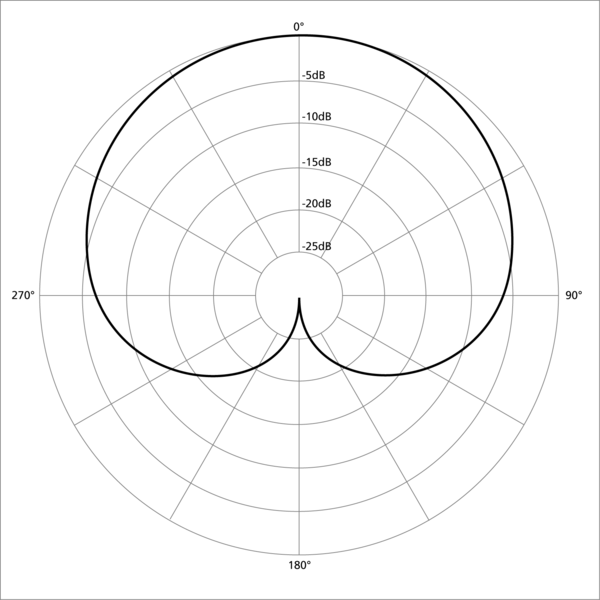
\includegraphics[width=2.5in]{cardiod}
    \caption{Cardioid Pattern response for directional hearing aids. $90^o$ represents the area directly in front of the user}
    \label{fig:cardiode}
\end{figure}


The issue with the beamforming hearing aids is that the sensitivity of the hearing aid drops off at low frequencies, like 1000 Hz \cite{thompson} . In order for the beamforming hearing aid to accommodate this situation, additional gain must be implemented in the hearing aid to hear low frequencies. However, additional gain comes at the cost of internal noise in the hearing aid, which is unwanted \cite{thompson}.

As mentioned above, all current solutions have a flaw that hampers the user’s use of their respective hearing aid. Kochkin  found that a quarter of individuals who own hearing aids but do not use them cite poor performance amid background noise as the primary reason \cite{kochkin}.
Further, as is shown by the polar of the directional hearing in Figure \ref{fig:cardiode}, many current directional solutions are dependent upon the listener physically looking at a target to obtain maximum amplification. However, this is often not the case in an actual conversation. There are many instances where a participant in a conversation may not be actively looking at other participants, such as when they are looking at a television, or moving through the room. In these scenarios, a listener’s ability to perceive the conversation should not be hindered by head position.



\subsection{Requirements}

Noting the two above scenarios, we have proposed a hearing aid system that allows an elderly user:

\begin{enumerate}
    \item To selectively attenuate or amplify nearby human targets within an indoor space, -essentially giving the user the ability to “mute” or “turn the volume up” on individuals within the room.
    \item To move about the room without negatively affecting the amplification of their conversation
\end{enumerate}

We achieve both of these goals using beamforming through a stationary array of microphones within the room, a process that we will describe in detail in Section II.


\subsection{Specifications}

The specifications for the hearing aid system are summarized in Table 1: \\

\begin{table}[htb!]
    \centering
    \begin{tabular}{|l|l|}
    \hline
    Specification  & Value  \\
    \hline
    Array Width	& $<2$m \\
    Target Identification Range & $>20$ft \\
    Angle of Operation & $30^o$ to $150^o$ \\
    Maximum Number of Targets &	$>4$ \\
    Beamwidth &	$<15^o$ \\
    Bandwidth &	600 – 2400 Hz\\
    Delay & $<300$ms \\
    \hline
    \end{tabular}
    \caption{Specifications for Device}
    \label{tab:specs}
\end{table}



\textbf{Size and Range of Device:} To formulate our specifications, we made the assumption that the system will be operating within a user’s home in a space reserved for entertaining guests, such as a family or living room. Considering a 20’ x 20’ living room, this assumption provides the maximum distance that the system must identify and listen to targets, as well as the maximum allowed size of the system.

Within the relatively small space of a living room, it is important to ensure that any potential device does not disrupt the normal daily life of any occupants. We desire a wall-mounted system to leave as much floor space for the occupant as possible. The system should also not overtly draw attention to itself and dominate the room. To accomplish this, we set a device size limit of 2 meters in length, about the size of a large hanging piece of artwork.

\begin{figure}
    \centering
    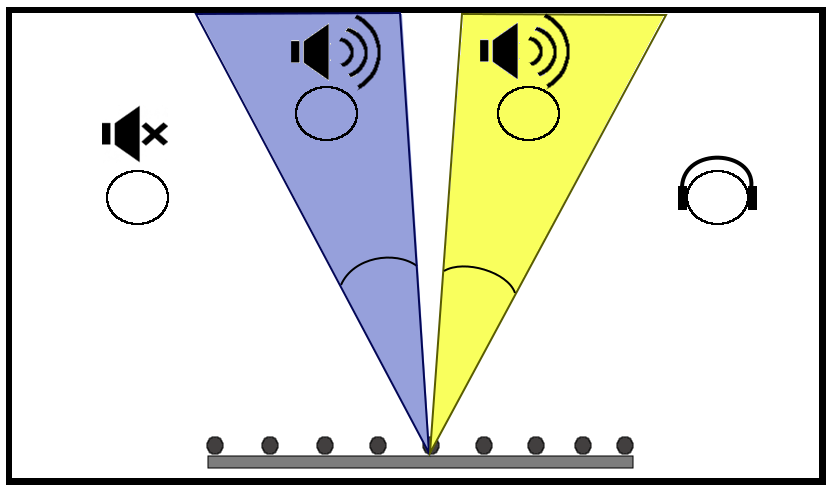
\includegraphics[width=3in]{beams}
    \caption{Desired behavior for our system. A wall mounted device is able to selectively listen to multiple targets within the room for a listener, here wearing headphones}
    \label{fig:beams}
\end{figure}

\textbf{Beamwidth:} To effectively isolate the output of sound sources, we must be able to encapsulate each target within distinct, non-overlapping beams, as seen in Figure \ref{fig:beams} If each target is centered within a beam, then the 3dB beamwidth of that beam must not intrude into the 3dB beamwidth of another beam. We considered a typical living room couch seat as the minimally spaced placement that any two people will be arranged within the room, as seen in Figure 2. If a typical couch cushion is 25” in width, and the couch is 8’ from the wall, then the  minimum beamwidth is approximately $15^o$

\begin{figure}[!h]
    \centering
    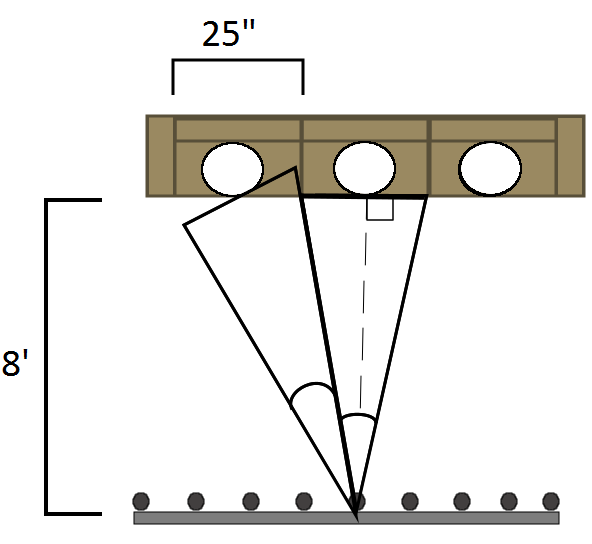
\includegraphics[width=3in]{find_bw}
    \caption{Finding the minimum beamwidth needed to encapsulate targets within individual beams}
    \label{fig:find_bw}
\end{figure}

\textbf{Bandwidth:} In typical telephony applications, the transmitted human speech spectrum range is about 300 to 3300 Hz, in order to maintain intelligibility  \cite{polycom}. However, Section II will show that beamwidth may be gained by sacrificing bandwidth, so we limit ourselves to 600 – 2400 Hz. This is  similar to the 300 – 2700 Hz bandwidth used for long-distance telephone connections in the 1980s \cite{polycom}.

\textbf{Delay:} To provide seamless conversations, the delay between reception of sound and playback to the user must be minimal. The ITU G-177 specification for VoIP mandates a two-way delay of less than 300 ms \cite{itu}, so we used this number to provide an upper bound on delay.

\textbf{Angle of Operation:} For a wall mounted system, microphones must be able to target and listen over a wide range of angles to provide adequate coverage for the entire room. For a microphone array parallel to a wall, we would ideally want to isolate and amplify sound over a range of $180^o$. However, the nature of our signal processing method, beamforming, ensures that isolating sound from sources close to the extreme ends of this range is difficult (at $0^o$/$180^o$, ie. when a source is close to the same wall where the system is mounted).

\begin{figure}
    \centering
    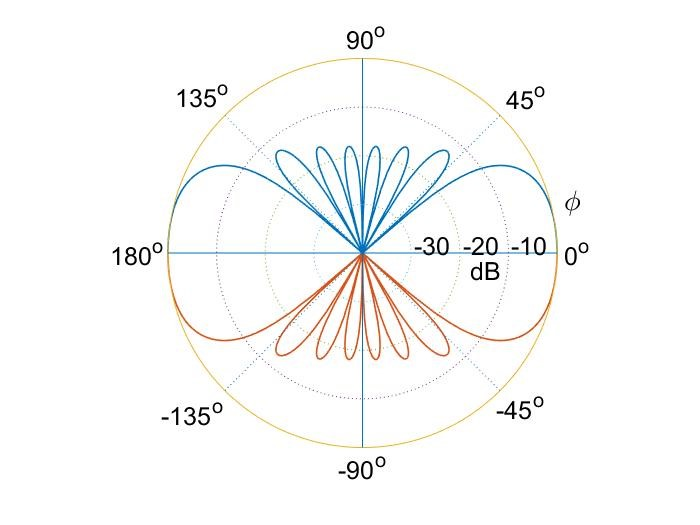
\includegraphics[width=3in]{endfire}
    \caption{This is the array response when the elements are steered toward $180^o$ or $0^o$. You cannot amplify one direction without also amplifying the other direction}
    \label{fig:endfire}
\end{figure}

For reasons that will be expanded upon in Section \ref{sec:mic_array} we cannot amplify targets at $180^o$ without also amplifying sound at $0^o$. This is called an "endfire" array response , and may be seen in Figure \ref{fig:endfire}.

We desire for the user to have individual control over each possible source of sound, so we have chosen to limit the angle of operation to $30^o$ to $150^o$ to avoid the endfire configuration. For our problem, this is a reasonable limitation, as most targets will be present at some point within the room, not hugging the wall of the device.




\section{Design}

\subsection{Overview}

Our approach to addressing this problem harnesses the power of audio beam-forming and mates it with an intuitive user interface.  This is enabled by a visual tracking system alongside a mobile app that allows intuitive user interaction for system control.  The beam-forming approach has been used several times before and is well documented.  Furthermore, our processing algorithm gives us a very low latency so that this system viable for real-time communication.

There is a long history of acoustic beamforming projects in the UMass ECE department \cite{sdp04}\cite{sdp06}\cite{sdp14}\cite{sauron}. Project Sauron from 2016 left behind a significant amount of valuable hardware, from microphones to a 16 channel ADC. To save on costs, we have aimed to utilize these features within our own project.

However, while using past hardware, we seek to improve upon the performance and usability of previous design projects. One of our aims is to automate the system as much as possible while allowing the user to control only what is relevant, specifically which individuals they would like to isolate and hear. The Microsoft Kinect plays a key role in allowing this automation with its ability to identify and map unique individuals. The mobile app displays this data and allows for user selection.  The software program performing the beam-forming processes the audio streams from the beam-forming array and outputs them to the user’s headset.  An overview of this system is shown in Figure 3.

\begin{figure*}[!htb]
    \centering
    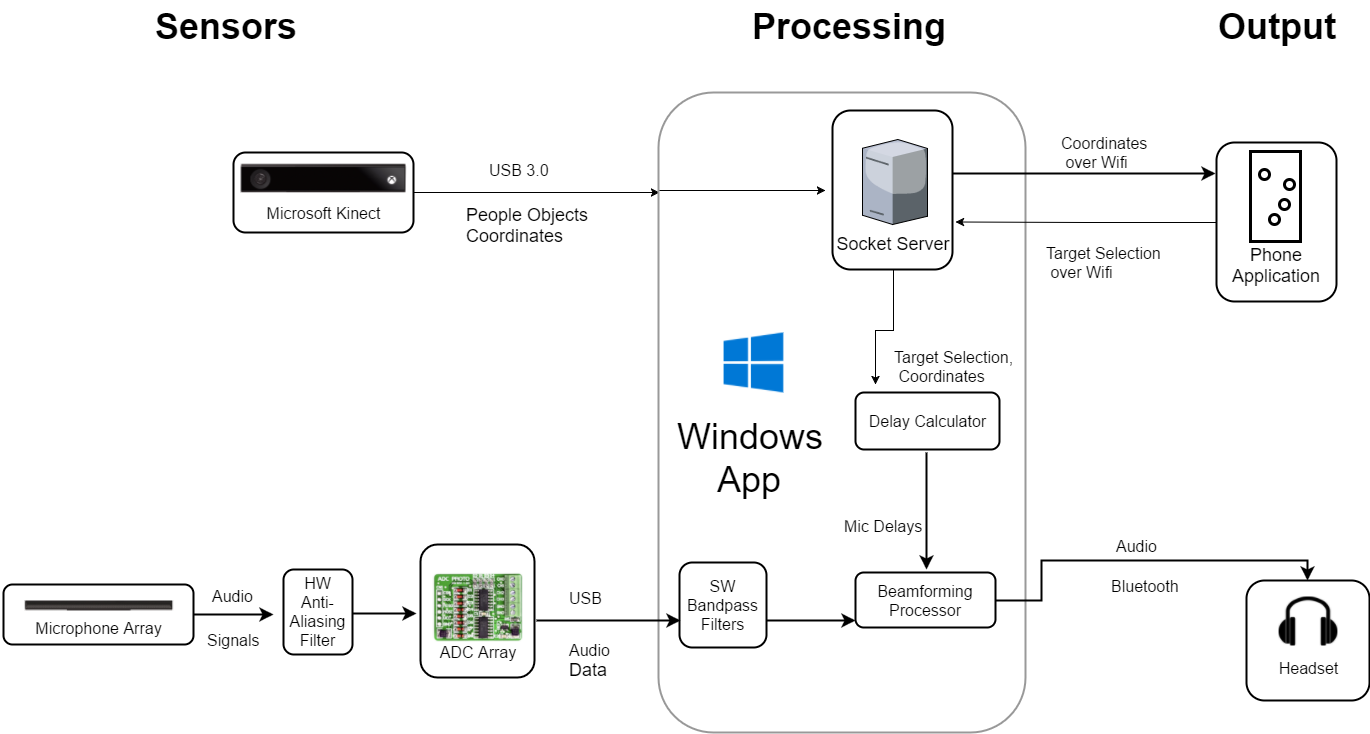
\includegraphics[width=6in]{system_block}
    \caption{Caption}
    \label{fig:my_label}
\end{figure*}
% needed in second column of first page if using \IEEEpubid
%\IEEEpubidadjcol

\subsection{Microphone Array}
\label{sec:mic_array}
The microphone array is the method through which sound is sampled spatially from the environment. Through classes such as ECE 313 and ECE 563, we are familiar with how an analog signal may be sampled in time by a set sampling period. An array of elements displaced by a set distance d samples the same signal with a relative phase shift between elements. By adding the output of each element together, signals from certain directions are added constructively, while signals from other directions are added destructively.

An array of elements with identical radiation patterns can be described by a term called the array factor, which for a one-dimensional linear array of n elements can be written as:

\[
A(\phi) = a_0 + a_1e^{jkd\cos(\phi)} + ... + a_ne^{jnkd\cos(\phi)}
\]
\begin{equation}
    A(\phi) = \Sigma_na_ne^{jnkd\cos(\phi)}
\end{equation}

Where d  is the distance between microphones, k  is the wavenumber of an incoming wave, $phi$ is the direction of propagation for the sound wave,  and $a_o$ … $a_n$ are complex coefficients \cite{sophocles}. This sum of complex exponentials completely describes the geometry of the array, with each term representing the relative phase shift resulting from the time that it takes for a wave to propagate from element to element.

\begin{figure}[!htb]
    \centering
    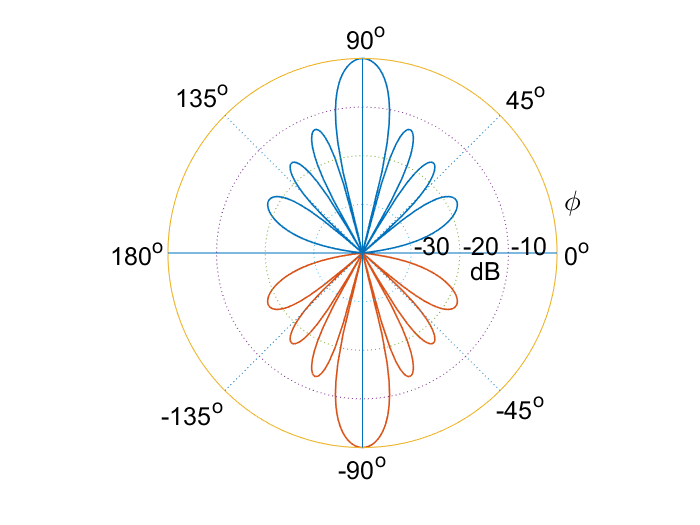
\includegraphics[width=3.5in]{broadside}
    \caption{Array Power gain $|A(\phi)|^2$ for an array of 8 elements, spaced one-half a wavelength apart, with each microphone equally weighted}
    \label{fig:broadside}
\end{figure}

The array factor has a dramatic effect on the directivity of the array.  For a wave incoming at a direction of $\phi$, if each element has an identical power gain of $G(\phi)$, then the gain of the entire array system $G_{tot}(\phi)$ is \cite{sophocles}:

\begin{equation} \label{eq:pattern_mult}
G_{tot}(\phi) = |A(\phi)|^2G(\phi)
\end{equation}

For example, Figure \ref{fig:broadside} contains a polar plot of the term $|A(\phi)|^2$ for a linear array of 8 elements, with coefficients $a_0 = \ldots = a8 = 1/8$, meaning that each element is equally weighted. In this scenario, the maximum power gain occurs when a wave is arriving perpendicular to the linear array, at $90^o$, also known as broadside. Intuitively, this is the direction where all microphone inputs add together in-phase.

By changing the coefficients $a_0 \ldots a_n$  to a set of complex exponentials, each sampling element provides a phase shift (i.e. a time delay) to the signal that it is sampling.  The direction of the main beam in the polar plot of $|A(\phi)|^2$ can be translated to another direction, called the steering angle. Figure 5 displays the array pattern for a beam aimed $35^o$ from broadside.

\begin{figure}[!htb]
    \centering
    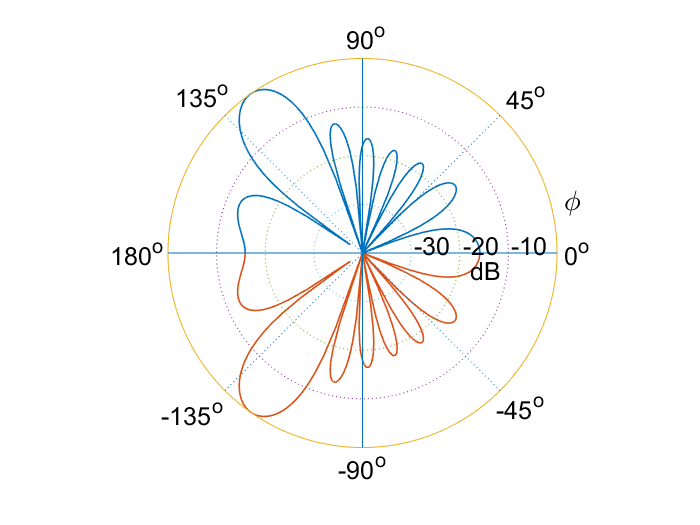
\includegraphics[width=3.5in]{steered}
    \caption{Array Power gain $|A(\phi)|^2$ for an array of 8 elements, steered towards $125^o$}
    \label{fig:steered_aliased}
\end{figure}

From (\ref{eq:pattern_mult}), we can see that there are two terms affecting the power gain polar pattern of our linear array:

\begin{itemize}
	\item $G(\phi)$ – determined by the microphone selection
	\item $|A(\phi)|^2$ – determined by the geometry of the microphone elements
\end{itemize}

By optimizing both of these terms, we can minimize the beamwidth of the array, and meet our specifications

\subsubsection{Microphones}

For microphone selection, we had access to the 16 omnidirectional ADMP510 MEMS microphones used in the SDP 16 beamforming project.  As the SDP 16 team noted, this particular model of microphone has a relatively linear frequency response within the frequency band targeted by our system \cite{sauron}.

\begin{figure}
    \centering
    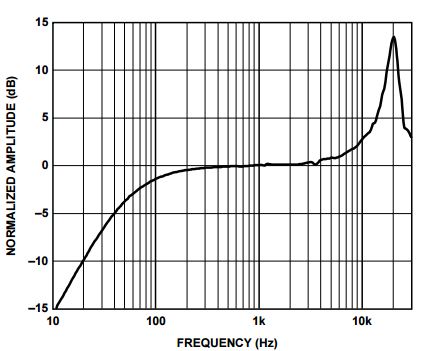
\includegraphics[width=3.5in]{mic_response}
    \caption{Frequency response for the ADMP510 microphones. Note the flat response over the targeted band 600 – 2400 Hz}
    \label{fig:mic_response}
\end{figure}

Given this property of the microphones, we decided to use SDP16’s microphones within our own design, to ensure that all frequencies within the targeted band are amplified equally. However, as we are receiving these microphones used, we will need to complete a verification procedure on each microphone, to ensure that it is still functioning after storage. To accomplish this calibration procedure, we will record low, medium and high frequency tones on each microphone, and then play each tone back. If the playback tone matches the original tone, then we can verify the microphone as functional.

Note that these microphones are omnidirectional, so tones are uniformly amplified in terms of direction. Thus,  (\ref{eq:pattern_mult}) simplifies to:

\begin{equation}
\label{eq:gain_simpl}
G_{tot}(\phi) = |A(\phi)|^2
\end{equation}

\subsubsection{Array Geometry}
As (\ref{eq:gain_simpl}) shows, the array factor is the only term that determines the directivity of the array. Therefore, in order to optimize the beamwidth, we need to select an optimal microphone geometry.

Orfanidis shows that for a uniform linear array, the 3dB beamwidth may be approximated as \cite{sophocles}:

\begin{equation} \label{eq:bw}
\Delta3dB = \frac{0.886\lambda}{\sin(\phi_0)Nd}b
\end{equation}

Where $\phi_0$ is the steering angle, $\lambda$ is the wavelength of tone, N is the number of microphones, d is the microphone distance, and b is a factor dependent on the weighting applied to each microphone.

 (\ref{eq:bw}) shows that beamwidth will increase as the beam is steered towards 0 or $180^o$, and as frequency decreases. This creates an issue for our beamformer, as it means that different frequencies within the human speech spectrum will produce different beamwidths.

Increasing d or N will decrease beamwidth, but the distance between microphones cannot be increased beyond $\lambda$L/2, where $\lambda$L is the largest wavelength within the targeted frequency band. This is the Nyquist criteria for spatial sampling through arrays, analogous to the Nyquist frequency for sampling in time \cite{sophocles}. If the Nyquist criteria is exceeded, then additional beams will appear that are equal in magnitude to the main beam. This is known as spatial aliasing, and an example may be seen in Figure \ref{fig:steered_aliased}.

With this knowledge in mind, we analyzed SDP16’s array. The SDP16 team used a nested array as pioneered by \cite{smith}, where the targeted frequency band was split into smaller bands, and then subarrays were constructed out of the 16 available microphones. By sharing microphones between subarrays, each subarray could be allocated 8 microphones.

\begin{table}[!h]
    \centering
    \begin{tabular}{|l|l|}
    \hline
    Band & Highest Wavelength to Mic Distance Ratio\\
    \hline
600 - 1000 & 0.617\\
1000 - 1700	& 0.69\\
1700 - 3500	& 0.72\\
\hline
    \end{tabular}
    \caption{Project Sauron Frequency Bands}
    \label{tab:sauron_bands}
\end{table}


However, for the SDP16 array, within each band, approximately half of the frequencies would exceed the Nyquist Criteria, as shown in Table \ref{tab:sauron_bands}:

\begin{figure*}[!t]
\centering
\subfloat[a]{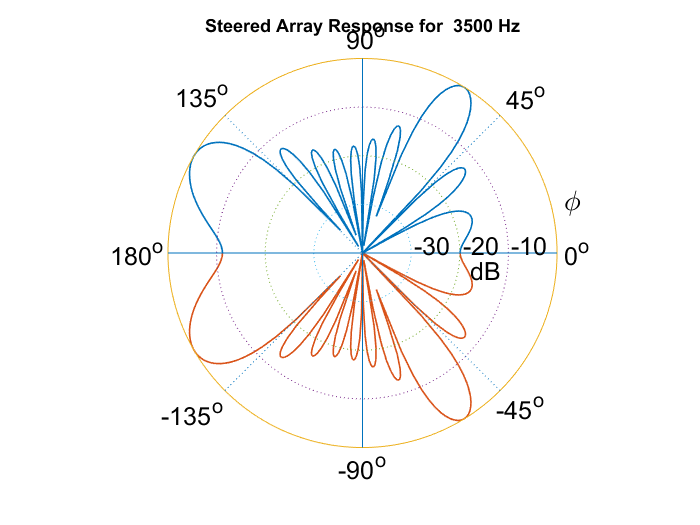
\includegraphics[width=2.2in]{steered_single}%
\label{fig_first_case}}
\hfil
\subfloat[b]{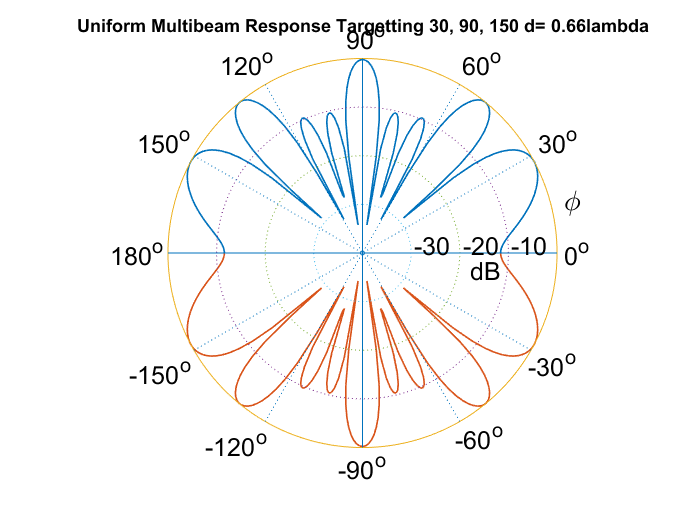
\includegraphics[width=2.2in]{steered_multi_old}%
\label{fig_second_case}}
\hfil
\subfloat[c]{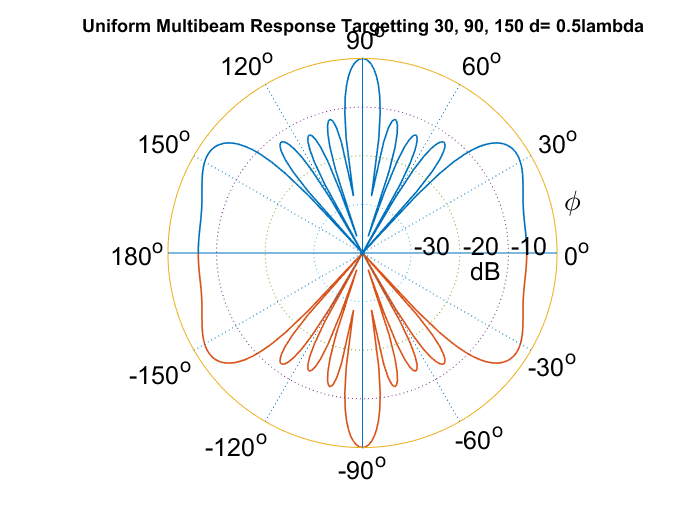
\includegraphics[width=2.2in]{steered_multi_earbeamer}%
\label{fig_third_case}}
\caption{The left plot shows the SDP16 arrays response to a 3500Hz signal when the array is steered to $150^o$, creating an aliased lobe at approximately $60^o$. The center plot shows SDP16’s array response when beamforming is performed in parallel, and aimed at 30, 90, and 150 degrees. The spatial aliasing at 135 and 55 degrees adds a significant amount of unwanted amplification to the field. The far right plot shows the highest frequency for the Earbeamer array, pointed at the same locations, with no spatial aliasing}
\label{fig:multi_beam}
\end{figure*}

\begin{figure*}
    \centering
    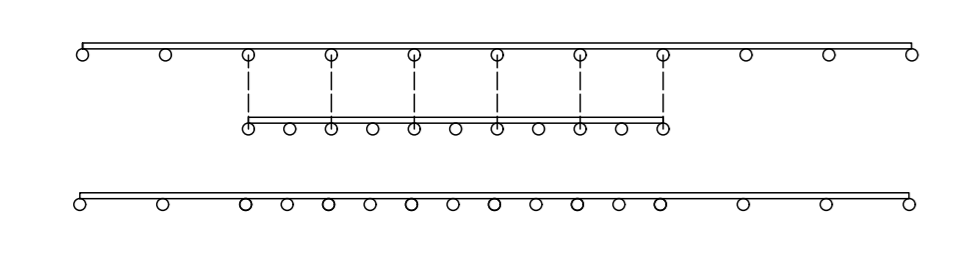
\includegraphics[width=6in]{array}
    \caption{ The Array Geometry for the new Earbeamer array. 16 microphones are shared between a [600,1200] band with d= 7cm, and a [1200,2400] band with d = 14cm}
    \label{fig:array}
\end{figure*}



Figure \ref{fig_first_case} and \ref{fig_second_case} demonstrate the negative effects of exceeding the Nyquist criteria. As our system implements beamforming in parallel, the spatial aliasing would add even more noise, as the additional beams will each produce an aliased beam.

To correct this issue, we divided the targeted frequency band into octaves, as Smith originally did. For a frequency band [$f_L$, $f_H$]:

\begin{itemize}
\item	For each octave [$f_{iL}$, $f_{iH}$], a subarray was created with microphone distance di = 1/(2$f_{iH}$), to avoid aliasing
\item	Each successive subarray had a microphone distance $d_{i}$ = 2$d_i$-1, to share as many microphones as possible
\item	All subarrays were allocated the same number of microphones, to ensure that the array response to each band was identical
\end{itemize}

With these requirements, we could create three arrays targeting [600, 1200],[1200, 2400], and [2400, 4800] Hz. By eliminating the highest frequency band, we could increase the number of microphones allocated to the lower bands from 8 to 11 microphones. Internal tests among the team found that speech was still intelligible lacking the higher frequencies.

The array performance is summarized in the table below, for the best and worst cases frequencies:

\begin{table}[!h]
    \centering
    \begin{tabular}{|l|l|l|}
        \hline
        $d/\lambda$ & Steering Angle & Beamwidth  \\
        \hline
        $\lambda/4$  & 90 & 18.5\\
                     & 150 & 36.9\\
        $\lambda/2$  & 90 & 9.3\\
                     & 150 & 18.5\\
        \hline
    \end{tabular}
    \caption{Earbeamer Array Performance}
    \label{tab:earbeamer_performance}
\end{table}

As shown in Table 3, beamwidth suffers when the steering angle is directed towards its maximum angle of $150^o$. However, beamwidth in the regions directly in front of the array, from 60 to 120 degrees remains relatively close to the specification. This is likely the best performance we can achieve with our current 16 channel Analog to Digital converter. From Equation 4, the only way to narrow beamwidth further is to add more microphones, but that would require purchasing an ADC that is outside the range of our budget.

\subsection{Beamforming Algorithm}

Our beamforming algorithm uses a delay-sum technique, where a different time delay is applied to each microphone in the array before combining the signals together. By calculating the delays using the position we wish to target, we can align the phase of the signals sourced from that location causing constructive interference, thus theoretically amplifying the audio only from that location.

\begin{equation} \label{eq:beamforming}
y[n] = \Sigma^{M-1}_{m=0}x[n-m\tau]
\end{equation}

The beamforming algorithm was implemented using a pipelined approach in C++. The idea behind the pipelined approach is that we can be constantly reading in audio data, which has an I/O cost associated with it, while performing calculations on the previously received audio at the same time. This way, we would be given the sample length to perform all our calculations. We use 3 rotating buffers per microphone, reading from two of them, and writing to the third to minimize memory movements and have a seamless flow through the audio. Using a sample rate of 16kHz and a sample size of 1024 samples, each buffer would hold 64ms of audio data.

One of our concerns was the amount of time the beamforming calculations would take for a single beam. As we are interested in calculating multiple beams, it is important that we can perform the calculations much faster than the time each sample takes. After running tests on our beamforming algorithm, we calculated that on average it takes under 200us to perform the beamforming calculations for one beam, well under the 64ms we have.


\subsection{Anti-Aliasing Filter and ADC}
The purpose of the anti-aliasing filter block is to cutoff sounds after a certain frequency. This filter comes before the Analog to Digital Converter, a device that converts the signal from analog to digital before being sent to the computer.

We have two main requirements for the filter:  we desire a sharp attenuation drop at the cutoff frequency, and a delay response that does not interfere with the beamforming algorithm. The latter requirement is because the filter does not affect all frequency components equally; some frequency components may be delayed more than others. Since our beamforming algorithm relies on delaying microphone inputs, unintended delays can damage our ability to recover a desired signal when microphone outputs are added together.

\begin{figure*}[t]
    \centering
    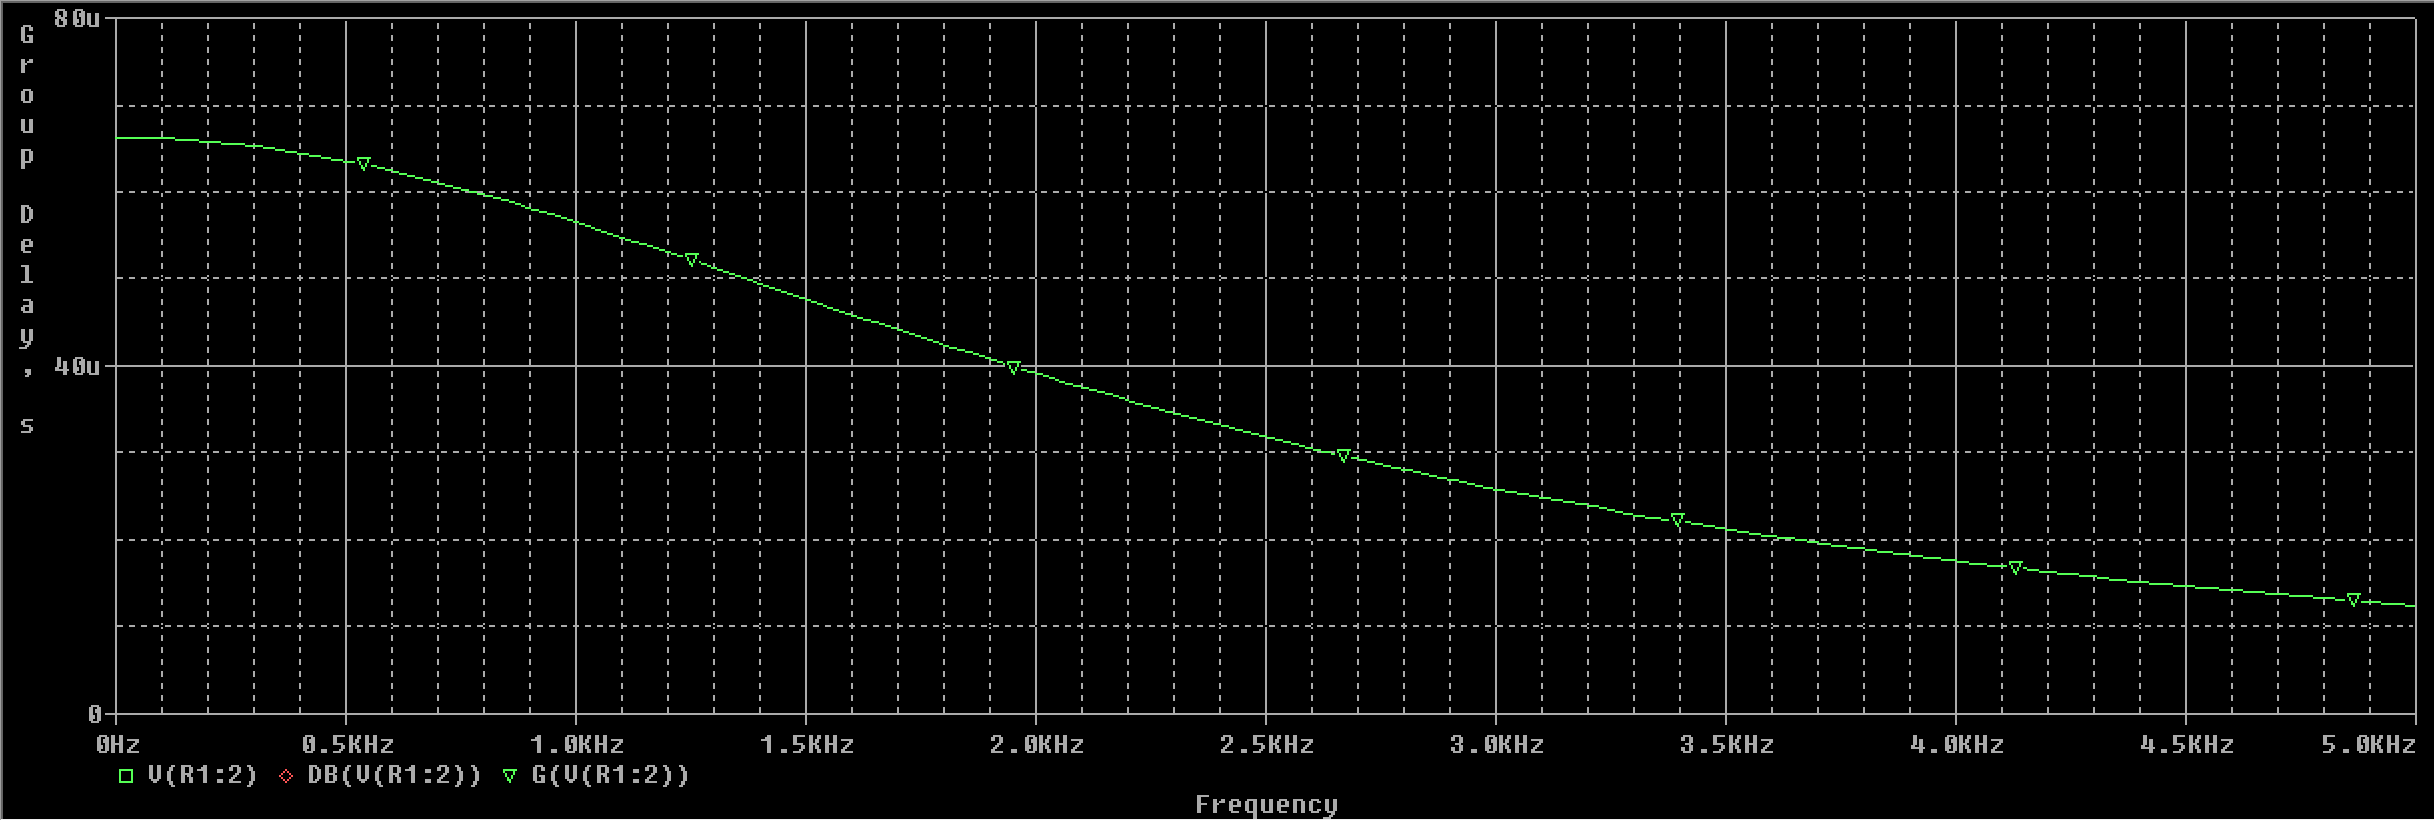
\includegraphics[width=6in]{group_delay}
    \caption{Group Delay of an RC Filter}
    \label{fig:group_delay}
\end{figure*}
\begin{table*}[t]
    \centering
    \begin{tabular}{|c|c|c|c|c|}
    \hline
        \textbf{Low Pass Filter} & Chebyshev Filter & Butterworth Filter & RC Filter & Linear Phase Filter\\
    \hline
            \textbf{Change in Group Delay}, $\mu$s & 793.75 & 173.53 & 33.15 & 0.12\\
            \hline
    \end{tabular}
    \caption{Comparison of Group Delay across Various Filter Configurations}
    \label{tab:group_delay}
\end{table*}

\begin{figure*}[t]
    \centering
    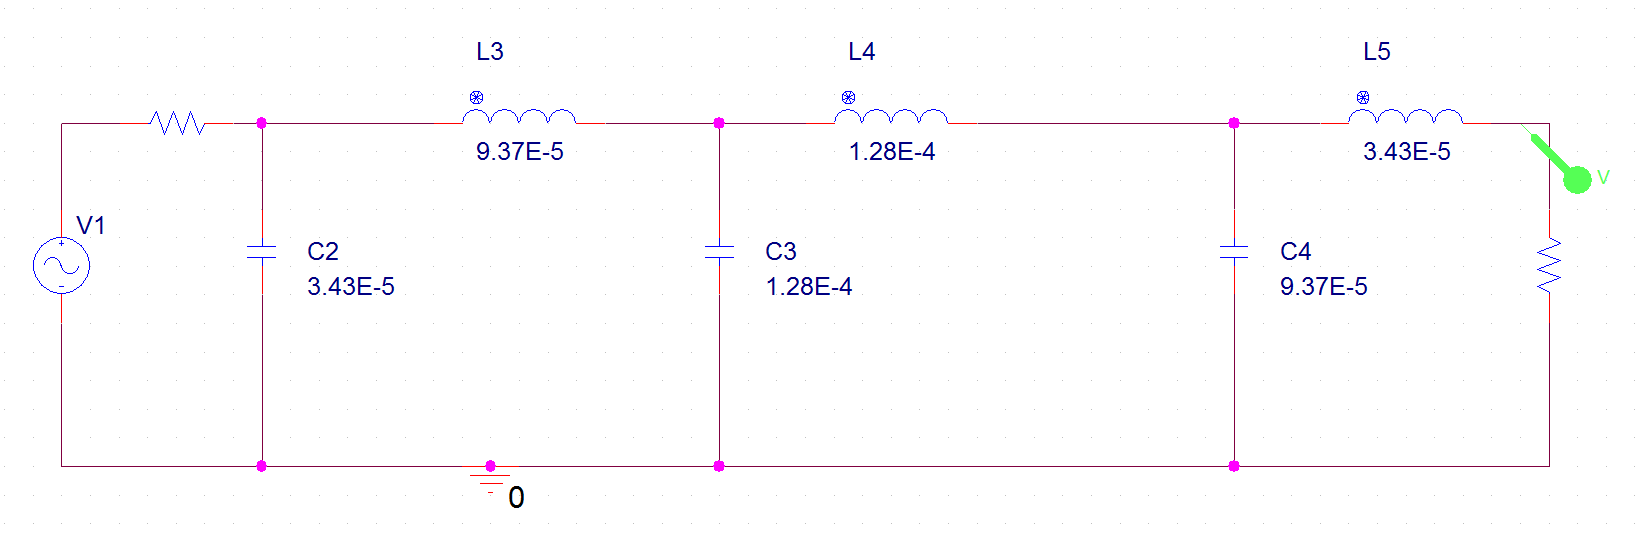
\includegraphics[width=6in]{filter}
    \caption{Butterworth Antialiasing Filter}
    \label{fig:filter}
\end{figure*}

We can evaluate the effect of the filter on the delay of various frequencies by measuring the group delay.  Group delay “… is the rate of change of transmission phase angle with respect to frequency” \cite{group_delay}. Figure \ref{fig:group_delay} gives a helpful visual of the appearance of group delay over the human speech frequency. This is the group delay of the RC filter plotted through PSPICE. Our cut-off frequency was 2.4 kHz because we want to use frequencies 2.4 kHz and below. The goal is to have no change in group delay in the pass band (0-2.4 kHz).

The highest possible sampling rate we can achieve with our ADC is 16000 Hz, or about 1 sample every 62$\mu$s. We cannot allow the group delay to exceed this value, or else the audio may become distorted after beamforming. In this case, the biggest change of delay in the pass band was 33.154us because of the change in group delay from 0 to 2.4 kHz. Other types of filters affect the drop off in attenuation and group delay differently from one another.

Through SPICE, we explored and simulated multiple filters for the microphones that applied to our requirements. Rather than building an RC series filter which gives a 3dB drop off at the desired cutoff frequency, it is preferred to have a sharper drop off at the cutoff frequency. There are well documented filter designs that can achieve sharper cutoffs using capacitors and inductors \cite{pozar}. In order to use these types of filter, we use a method called the Insertion Loss Method. This method is designed to combine capacitors and inductors on a circuit board in order to give the designer more control of filter’s attributes, like attenuation drop off and group delay.

The two filters that use the Insertion Loss method for sharp attenuation drops are the Butterworth filter and the Chebyshev filter. The Butterworth filter, as shown below in the figure, does not drop off in attenuation until we reach the cutoff frequency. The drop off in attenuation is linear after the cutoff frequency. The Chebyshev filter, a filter built in the same fashion as the Butterworth filter, offers a sharper drop off in attenuation at the cutoff frequency \cite{pozar}. However, as mentioned before, the greater the change in group delay in our desired passband, the bigger the interference with the beamforming algorithm. We therefore took a look into the linear phase filter. The linear phase filter, another circuit using the Insertion Loss method, can achieve a very good delay response at the expense of a very slow attenuation drop off at cut off frequency. Table \ref{tab:group_delay} shows the changes in group delay when having a cut off frequency of 2.4 kHz.

 Before MDR, the initial approach to the hardware filter was to have a cut off frequency at 2.4 kHz, because that is the frequency band we need for the project. A suggestion made by Professor Kelly was to design the hardware filter that achieves a drop off in attenuation at 8kHz , because the target frequency band we want to use is from 0 to 2.4kHz. The group delay does not affect frequencies far away from the cut off frequency. Once the filtered signal is sent to the analog to digital converter, the signal would be sampled at 15 kHz. From there, we can use a software filter to extract only the human speech frequency spectrum. Since MDR, we have decided to use the simple RC filter to eliminate aliasing, due to its favorable group delay performance.



\subsection{Xbox Kinect}

A key component of our hearing aid system is the ability to identify targets within the room, and determine the location of each target relative to an array of microphones. These coordinates are used to dynamically aim our beamforming algorithm as targets move about the room. To accomplish this, we needed a robust computer vision system with a depth sensor that had adequate range to cover a typical living room. The Microsoft Kinect for the Xbox One fulfilled these requirements.

The Kinect uses a Time-Of-Flight system to gauge depth. An infrared emitter emits pulses of infrared light, and an infrared sensor records when the pulse is reflected back. By recording the time required for the reflection to arrive, the relative distance of a point in space may be calculated. Using this system, the Kinect is able to maintain an effective range of 0.5 to 4.5 meters \cite{kinect_spec}, which more than meets our minimum range specification of 20 feet. Further, the TOF system used in the Kinect for Xbox one has been proven accurate to a depth of 1mm \cite{chen}, which is more than adequate resolution for aiming the beamformer.


\begin{figure}[!htbp]
    \centering
    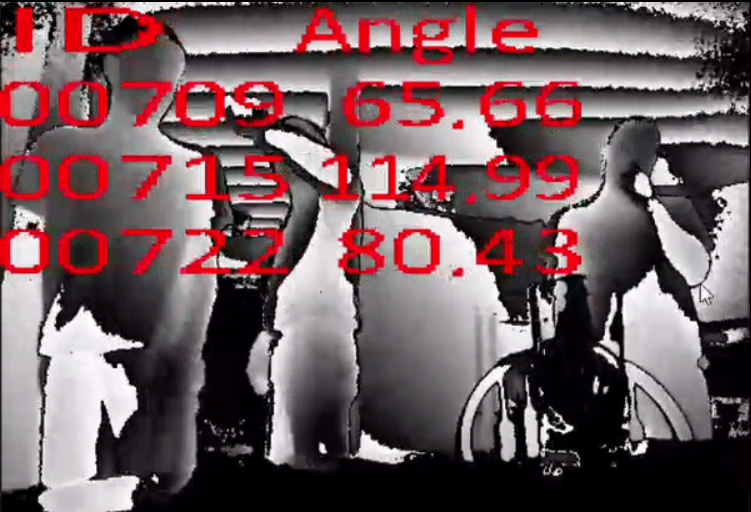
\includegraphics[width=8cm]{kinect_test}
    \caption{Screenshot of Kinect Demo for MDR. Depth data returned from the Kinect is plotted to the screen, as well as the IDs and angular displacement of all tracked targets}
    \label{fig:kinect_demo}
\end{figure}

To test and demonstrate the skeleton tracking for our MDR, a program was written to extract coordinates from any target that entered the field of view, calculate the relative angle of that target to the Kinect, and display the angle on a screen. A screenshot of this application is shown in Figure \ref{fig:kinect_demo}

Through the course of this testing, it was found that the angle of view of the Kinect was only about $60^o$, as shown in Figure 16 of the Appendix. Originally, we intended to place the Kinect directly below the microphone array, so that the origin of the Kinect’s coordinate system would align with the center of the array. However, our specification requires that any target from a $30^o$ to $150^o$ degree angle be selectable. To accommodate this, we must offset the Kinect to have a better view of the room, and then translate the returned coordinates to a system with the array center at its origin.

\subsection{IPhone Application}

The phone application is the single point of interaction for the user.  It communicates with the central processing software running on the computer.  Web socket technology has been chosen to allow for communication between mobile application and computer application.  This is a versatile, platform-agnostic protocol that is supported on many platforms.  More importantly, it allows two-way communication in an arbitrary manner – either party can send a message to the other at any time.

\begin{figure}
    \centering
    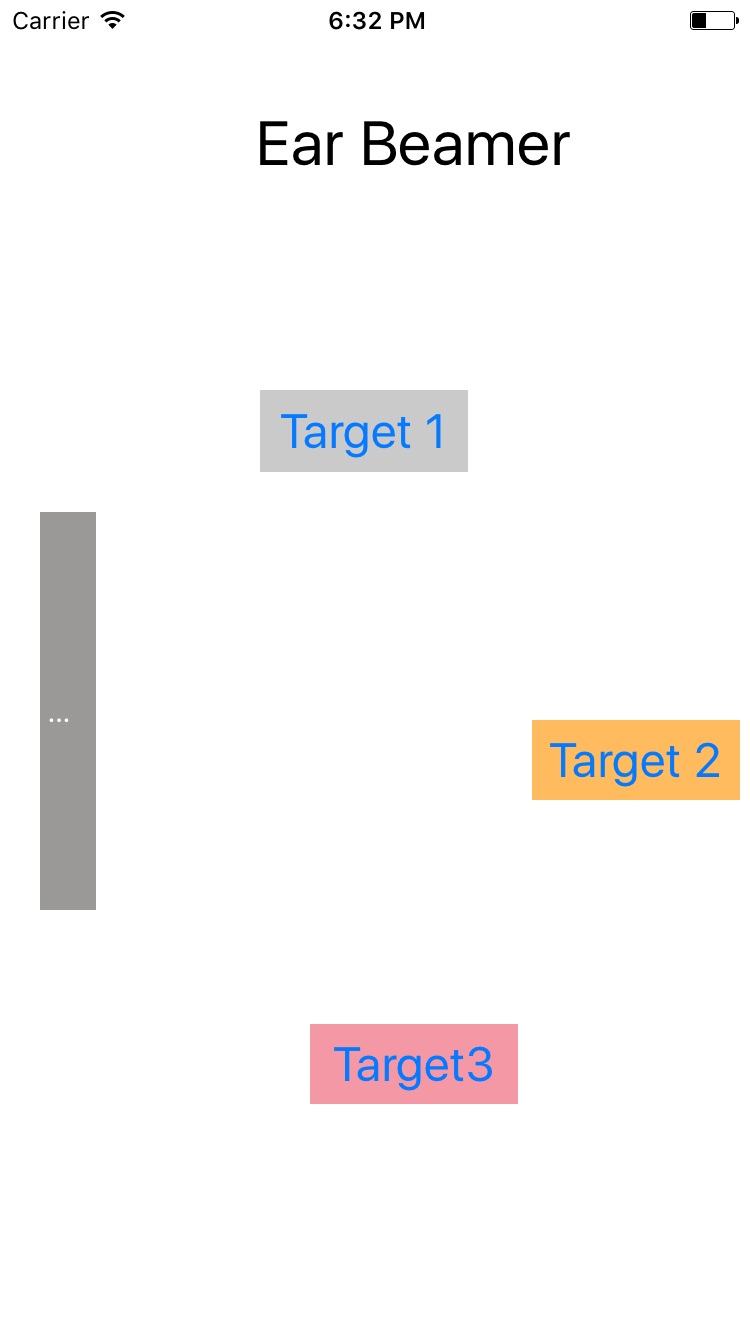
\includegraphics[width=2.5in]{app}
    \caption{Current Graphical interface for the application. Coordinates of identified targets are used to render representations to the screen}
    \label{fig:my_label}
\end{figure}

To create the application, an understanding of iOS application development is required, which is something that must be learned.  Specifically, development will be done in the Swift programming language using the Xcode IDE.  This was chosen as it is modern and well-supported, targeting interactive application development of all kinds. Software development techniques learned in the past have been and will be useful in learning this new platform and problem-solving during the development process.

The computer will run a server to stablish a connection with the application over a network.  This web socket server is created running on the node.js JavaScript environment.  It listens on a port to establish a link with clients, in this case the application. The socket.io engine was used to implement this functionality.  In addition to support for running the server with node.js, there is a socket.io library available for iOS Swift development which was integrated into the mobile application.

What the user sees is a graphical display of each target as shown in the figure.  The room layout on the display will have a fixed orientation, with a fixed reference point indicated.  When the target locations are updated on the main processing software, they will be sent by the server to this application.  These changes will be reflected by moving the position of each target indicator on the phone.  Each target displayed on the application can be pressed, and when it is, the phone sends this information to the server which alerts the system that a change in processing is required – either to enable or disable a specific target.


To test the functionality of this subsystem a mobile application was designed and created.  Then a server was set up and the application was deployed on an actual iPhone device.  Both devices were connected to the same WiFi network.  Pressing one of the target indicators on the app generated messages on the computer, reflecting which target was toggled.  This showed that arbitrary communication was possible between the two devices.  Further work must be done to make the app more interactive and dynamic.

\section{Project Management}

As each team member has unique professional and educational experiences, we divided the implementation of the project subsystems according to our particular strengths:

\begin{itemize}

\item Matteo Puzella is our sole Electrical Engineering major, with a particular interest in microwaves. He is applying his knowledge of filters to our project, as well as contributing to some of the more physical aspects of the project.
\item Aaron Lucia has an interest in system design, but also signal processing, and he is applying that to the beamforming algorithm.

\item Nathan Dunn has previously completed an REU that involved image processing, so he implemented the Kinect integration. He also completed research into the physics and dynamics of a beamforming array, helping with the design of the microphone array and the techniques of improving the beamforming.

\item Niket Gupta has developed an interest in mobile application development through past personal projects, and is working on the user interface with the mobile phone app, as well as figuring out the analog to digital conversion of the microphone signals.

\end{itemize}

With these assignments, the Ear Beamer team has successfully met its MDR objectives with deliverables beyond the initial plan shown in Figure 16 of the Appendix.  All subsystems have been shown to work successfully and the next objective is complete system integration.  With an initial focus on modelling beam-forming performance, we continued working to implement the hardware subsystems.  Currently the software and hardware subsystems are working successfully with synthetic inputs, without communication with other parts of the system directly.  They are all reading or processing data appropriately but must be patched together before the system will be fully functional.

Members of the Ear Beamer team have been assigned specific roles as shown in the figure, but continue to assist each other as needed. Weekly team meetings and adviser meetings help facilitate continued progress.  In addition, the team communicates frequently using a chat application called Slack, with occasional Skype group video calls.

The Ear Beamer is proceeding on schedule. We plan on having a working product and be able to present it for CDR in March. After CDR, we plan to implement Chebychev weighting on microphones and prepare for demo day in May. The full schedule for completing the project is shown in Figure 17 in the Appendix.

\section{Conclusion}

Currently, we have many of the subsystems working on their own, and we must now tie them together. We have planned for this, and are now diverting our attention to the modules of our design that link together major functional units. This includes the implementation of software filters to separate sampled audio into discrete $[600, 1200]$ Hz and $[1200, 2400]$ Hz bands for furhter processing in the beamforming algorithm. We are also developing a query/response protocol to allow a socket server on our Windows application to transfer target data to and from the iPhone application.


Another ongoing task is physically building the anti-aliasing filters, connecting them to the 16 microphone outputs, and running our beamforming algorithm on actual data. We anticipate encountering issues here, as most of our subsystems have been tested with simulated data, and we expect that real-world data might cause variances in our results.

For example, while our beamforming algorithm works with simulated data, this is under the assumption of operating within an echoless environment. In our model, sounds only travel away from the point that they originated. In reality, once a sound contacts a surface, it follows the Law of Reflection, and is reflected at an angle equal to the angle of incidence \cite{hyperphysics}.

Sound reflections may cause sounds that a user wishes to amplify to instead be attenuated, or vice versa. This could significantly impact our project's performance at the April demonstration. We are actively investigating methods to bring our demonstration space in line with an ideal, echoless environment. This could include building and installing acoustic barriers made of sound absorbing foam.

\section{Acknowledgements}
We want to acknowledge the SDP 16 project Sauron team for their advice and use of some of their hardware from last year. We would also like to acknowledge our advisor, Professor Parente, for helping us to stay organized and on schedule, as well as Professors Kelly, Goeckel, Yang, and Tessier for their advice
on beamforming applications and planning our project.

% references section
\printbibliography



% if have a single appendix:
%\appendix[Proof of the Zonklar Equations]
% or
%\appendix  % for no appendix heading
% do not use \section anymore after \appendix, only \section*
% is possibly needed

% use appendices with more than one appendix
% then use \section to start each appendix
% you must declare a \section before using any
% \subsection or using \label (\appendices by itself
% starts a section numbered zero.)
%


\appendices
\section{}

\begin{figure*}[t]
\centering
\subfloat[a]{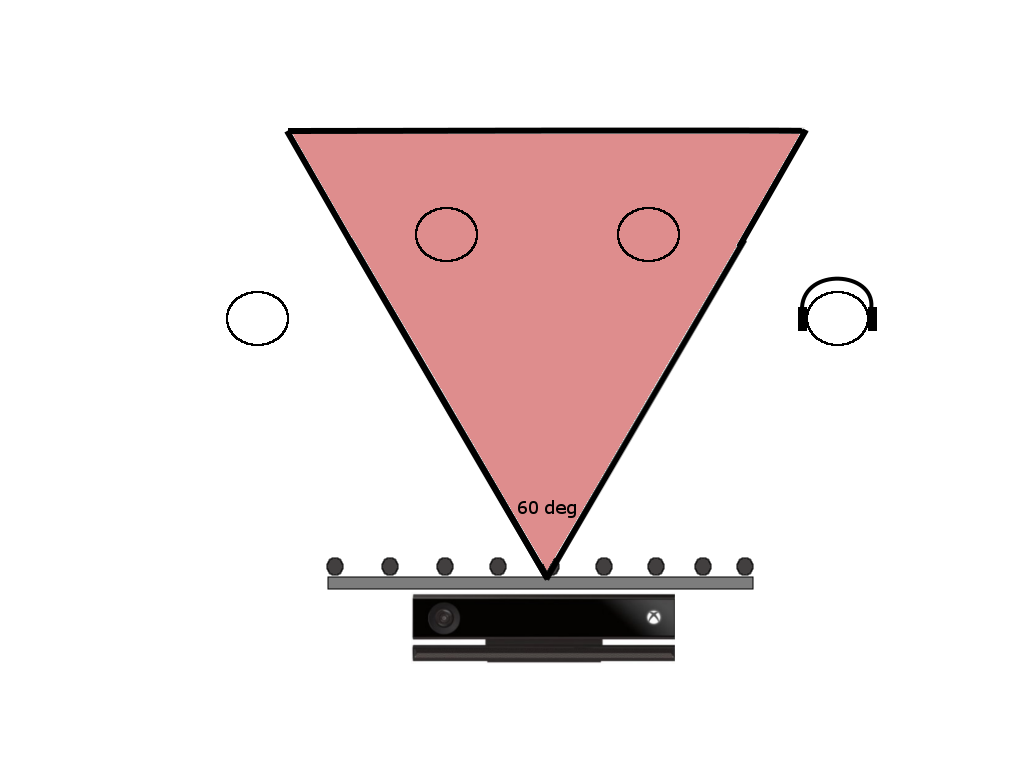
\includegraphics[width=3.7in]{kinect_view}%
\label{fig_kinect}}
\hfil
\subfloat[b]{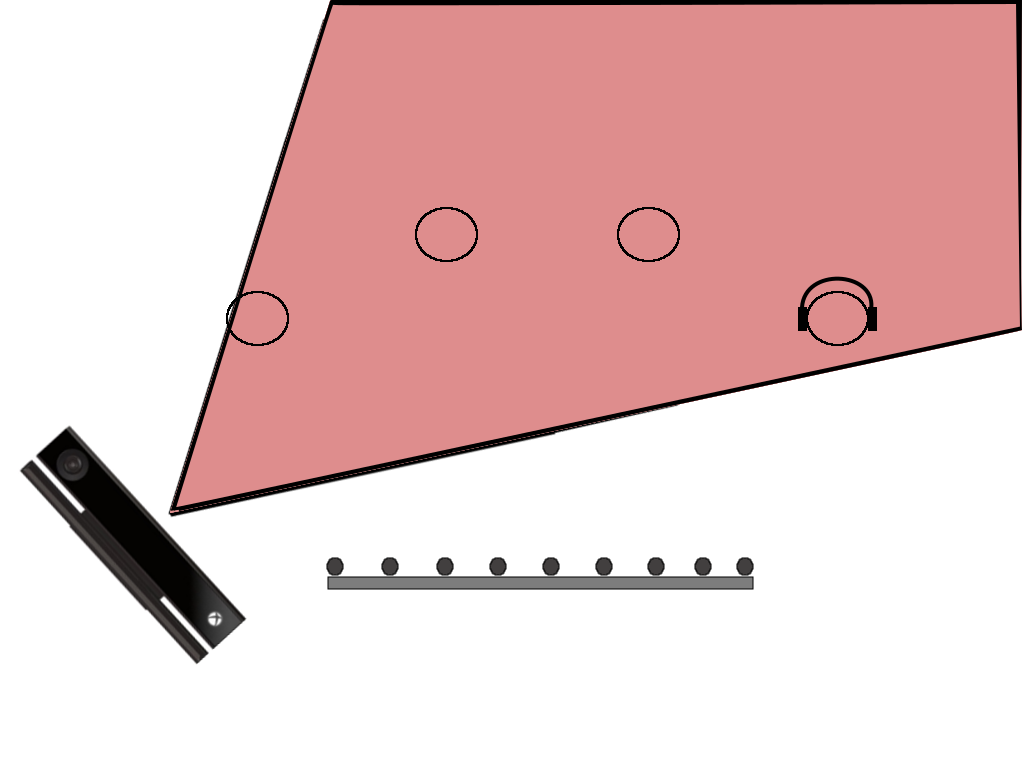
\includegraphics[width=3in]{kinect_view_steered}%
\label{fig_kinect_steered}}

\caption{The Angle of View is too narrow to adequately cover a room, so the Kinect must be offset from the microphone array to identify all possible targets}
\label{fig:kinect_straight}
\end{figure*}

\begin{figure*}[t]
    \centering
    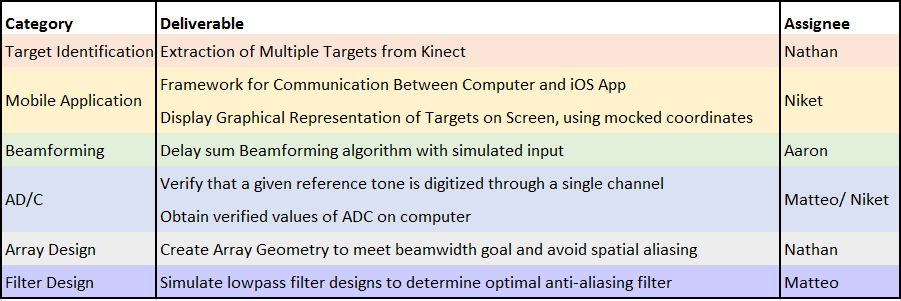
\includegraphics[width=6in]{mdr_deliverables}
    \caption{Caption}
    \label{fig:mdr_deliberables}
\end{figure*}

\thispagestyle{empty}
\begin{landscape}
\begin{figure}[]
    \label{fig:schedule}
    \centering
    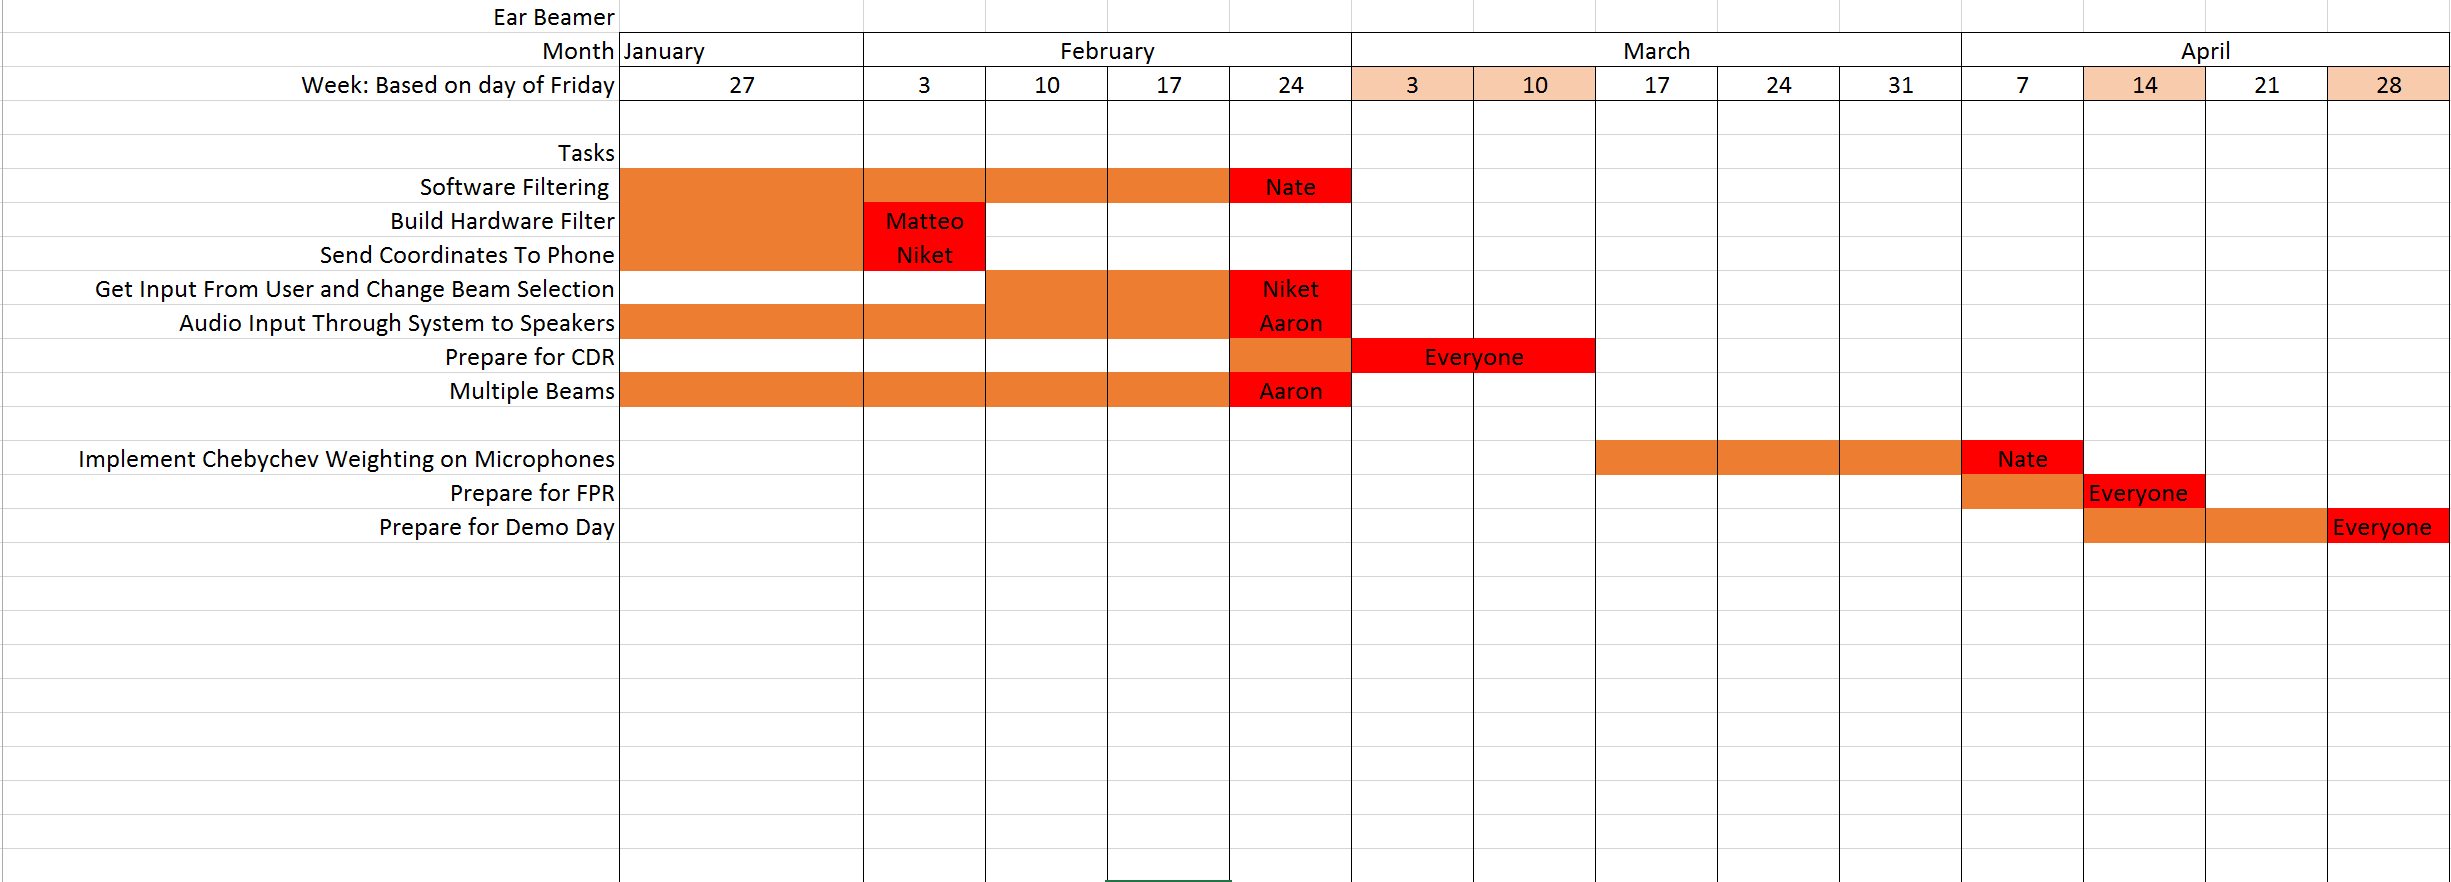
\includegraphics[scale=0.38]{schedule}
    \caption{Gantt Chart for the Remainder of the SDP Projet}
\end{figure}
\end{landscape}
% you can choose not to have a title for an appendix
% if you want by leaving the argument blank




% Can use something like this to put references on a page
% by themselves when using endfloat and the captionsoff option.
\ifCLASSOPTIONcaptionsoff
  \newpage
\fi



% trigger a \newpage just before the given reference
% number - used to balance the columns on the last page
% adjust value as needed - may need to be readjusted if
% the document is modified later
%\IEEEtriggeratref{8}
% The "triggered" command can be changed if desired:
%\IEEEtriggercmd{\enlargethispage{-5in}}



% biography section
%
% If you have an EPS/PDF photo (graphicx package needed) extra braces are
% needed around the contents of the optional argument to biography to prevent
% the LaTeX parser from getting confused when it sees the complicated
% \includegraphics command within an optional argument. (You could create
% your own custom macro containing the \includegraphics command to make things
% simpler here.)
%\begin{IEEEbiography}[{\includegraphics[width=1in,height=1.25in,clip,keepaspectratio]{mshell}}]{Michael Shell}
% or if you just want to reserve a space for a photo:


% You can push biographies down or up by placing
% a \vfill before or after them. The appropriate
% use of \vfill depends on what kind of text is
% on the last page and whether or not the columns
% are being equalized.

%\vfill

% Can be used to pull up biographies so that the bottom of the last one
% is flush with the other column.
%\enlargethispage{-5in}



% that's all folks
\end{document}
